\section{Projectresultaat}
Het doel van de stageopdracht is om een draadloze sensor-probe te ontwikkelen die gebruikt kan worden in een proof-of-concept. Deze probes moeten in staat zijn om met reeds geselecteerde sensormodules dissolved oxygen (DO) te meten. Deze informatie moet draadloos verzonden worden en moet op een manier weer teruggekoppeld kunnen worden aan de regelmodule van de bioreactor. Dit systeem moet ook geïntegreerd worden in een testopstelling die duidelijk moet maken of de gewenste betrouwbaarheid van sensoren met kabels ook behaald kan worden door de draadloze probe.

\subsection{Functies}
\begin{figure}[H]
	\centering
	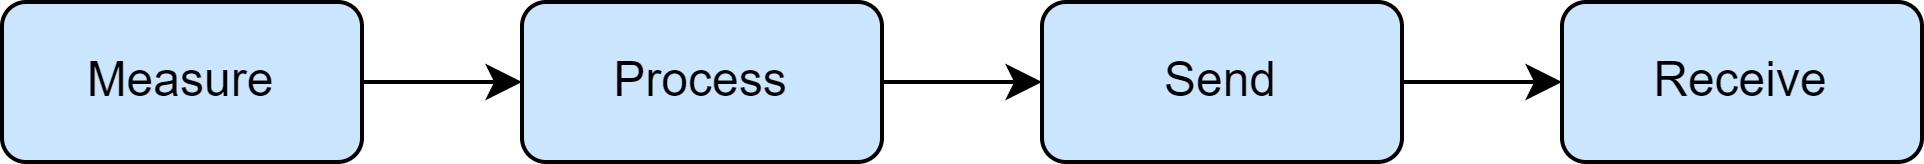
\includegraphics[width=0.60\linewidth]{graphics/function}
	\caption{Functies van het systeem}
	\label{fig:function}
\end{figure}
Het sensor systeem vervult vier functies; meten, verwerken, versturen en ontvangen. Aan de hand van een polarographic DO sensor wordt het DO level van de vloeistof bepaald. Er wordt een pakket opgesteld met alle waardes die de biocontroller moet ontvangen. 

\subsection{Systeemarchitectuur}
Als leidraad voor het vaststellen van systeemvereisten dient er een overzicht gemaakt te worden die duidelijk maakt uit welke (deel)systemen dit project bestaat en wat de scope van de ontwikkeling is tijdens dit project. Ook dient er duidelijk gemaakt te worden met welke bestaande systemen dit project te maken heeft, en in welke capaciteit. 

\subsubsection{Systems Engineering}
Aan de hand van Systems Engineering is er een overzicht gemaakt van het gewenste systeem. In figuur \ref{fig:sensor_bdd} is een Block Definition Diagram (BDD) van het gewenste systeem te zien.

\begin{figure}[H]
	\centering
	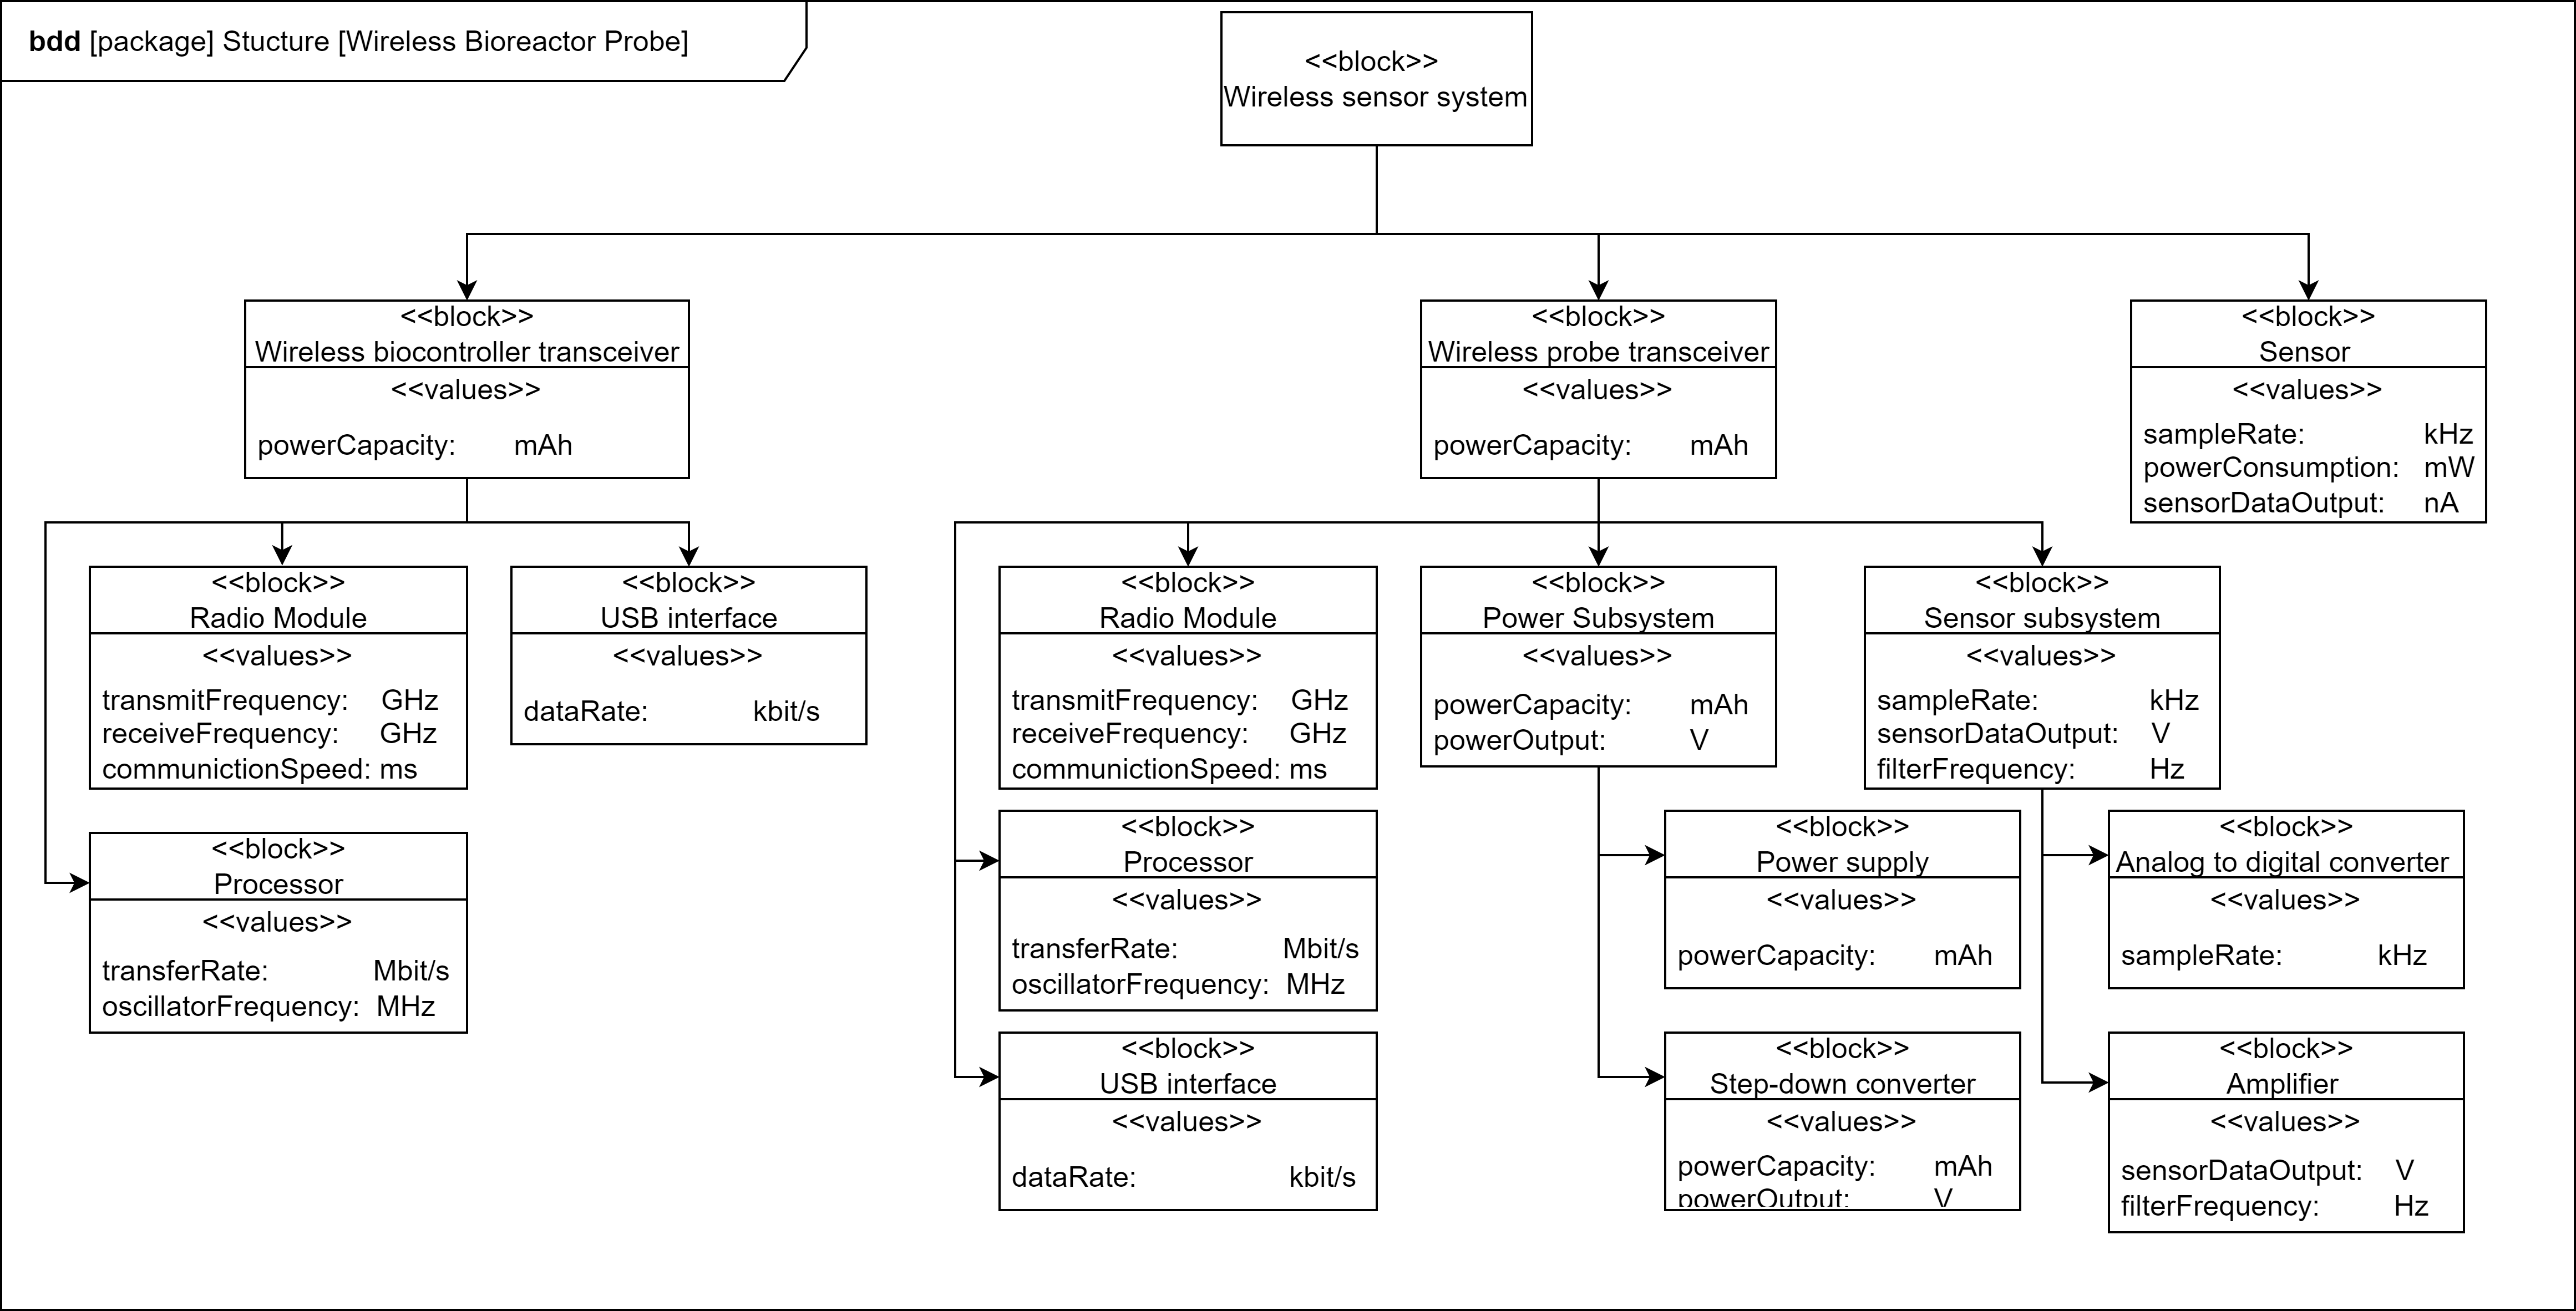
\includegraphics[width=1.0\linewidth]{graphics/sensor_bdd}
	\caption{Block definition diagram voor het draadloze bioreactor sensoren}
	\label{fig:sensor_bdd}
\end{figure}
In het BDD is te zien dat het wireless sensor systeem bestaat uit drie subsystemen: de biocontroller transceiver, de probe transceiver en de DO sensor. De biocontroller transceiver zal worden aangesloten op de biocontroller zodat het systeem draadloos kan communiceren met de DO sensor via de probe transceiver module. 

De biocontroller transceiver is een simpel systeem dat bestaat uit een draadloze module om met de andere probe te communiceren, een microcontroller om de data te verwerken en een USB interface om te communiceren met de biocontroller. 

De module voor de probe bestaat uit drie subsystemen: een draadloze module, een sensor module en een power systeem. Via de draadloze module wordt het sensor signaal versterkt, digitaliseert en verzonden. Het power subsysteem verzorgt de probe en de module van stroom. 

Het doel van de probe transceiver module is om de bestaande analog to digital systeem te verfijnen en uit te breiden met een draadloze module. Het wireless bioreactor sensor systeem wordt uitgerust met onder andere een processor om nodige sensor data te verwerken en de draadloze module aan te sturen.  

De probe wordt voorzien van een batterij als voeding van het systeem. In de eerste versie wordt het systeem nog niet ontworpen om de batterijen te laden. Zodra de batterij leeg is zal het verwisseld moeten worden. Tijdens het onderzoek en testen zal het duidelijk worden hoelang het systeem kan werken op een accu. Naast de optie om het systeem te voeden met een batterij zal het ook mogelijk worden gemaakt om het systeem aan de hand van een labvoeding te voeden of USB te voeden. Hoe dit precies wordt gedaan moet nog uitgezocht worden. 

\begin{figure}[H]
	\centering
	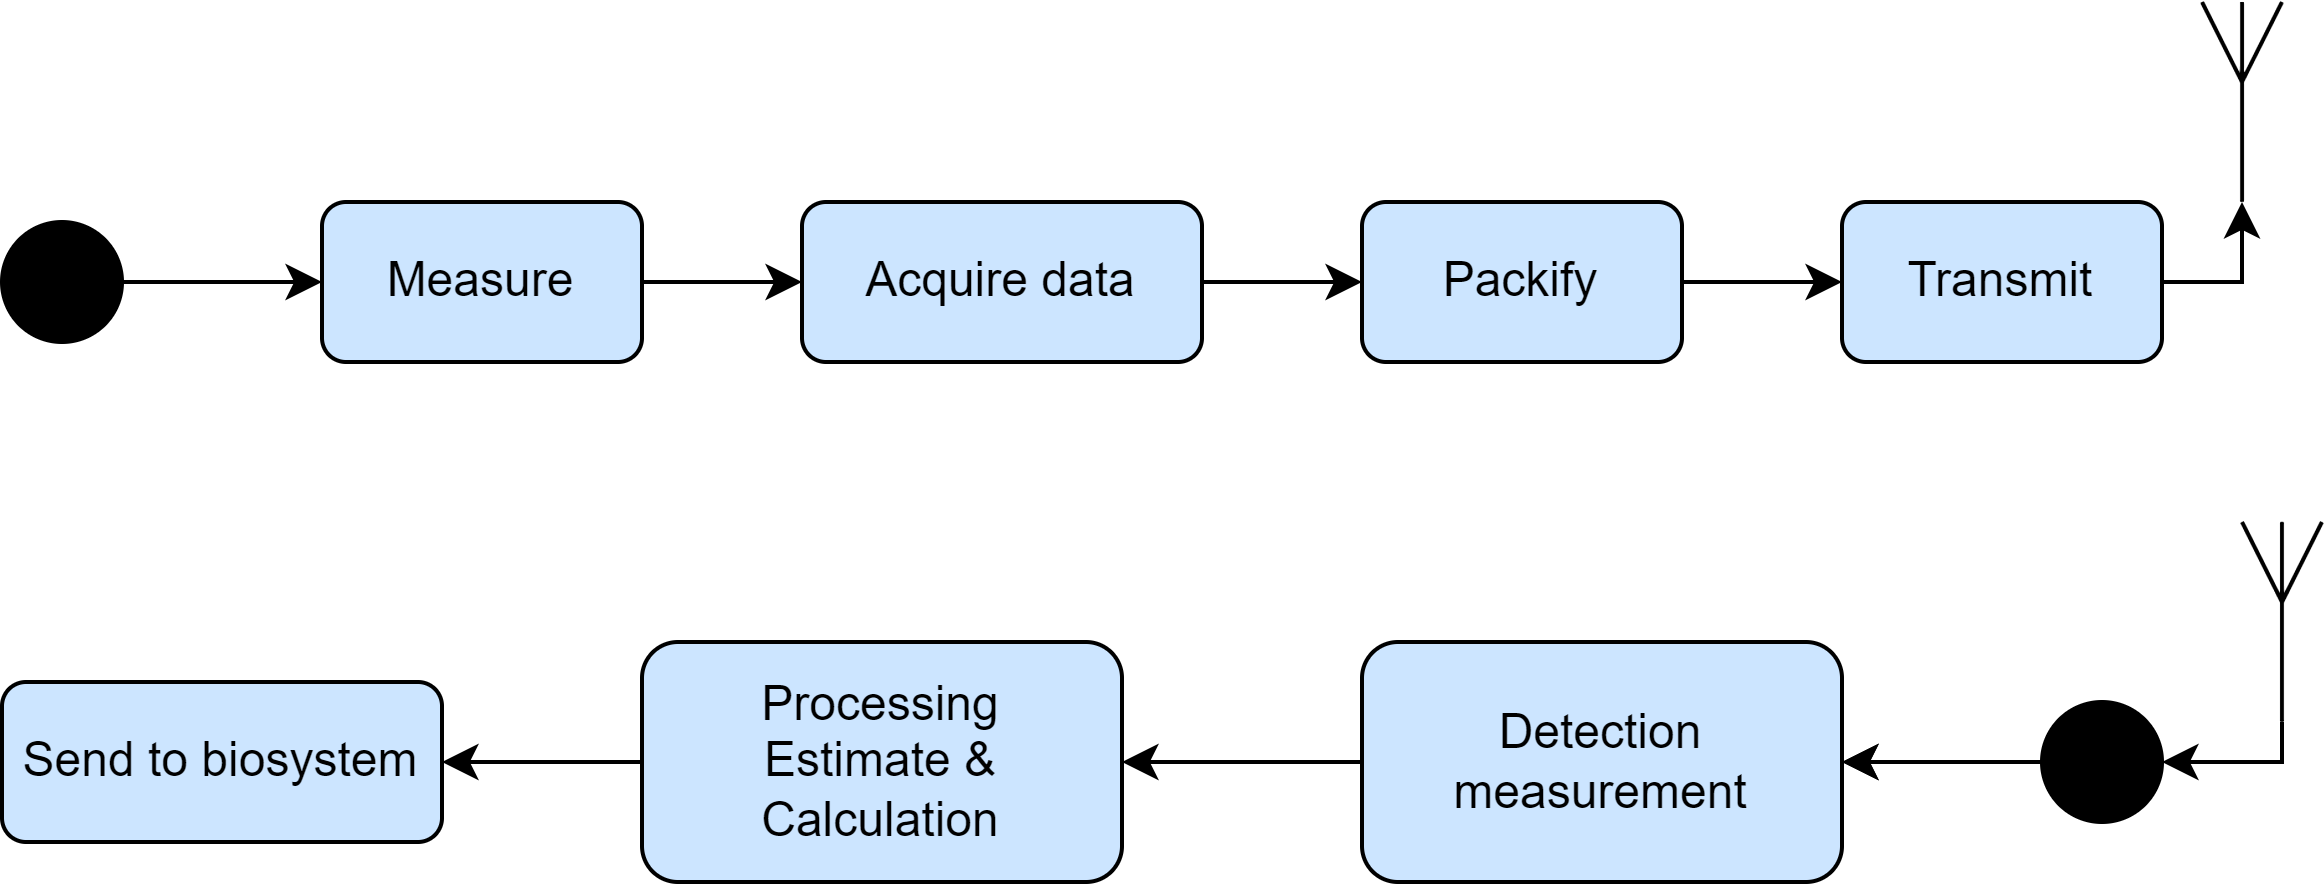
\includegraphics[width=0.60\linewidth]{graphics/probe_flow_simple}
	\caption{Flow diagram voor het draadloze bioreactor sensoren}
	\label{fig:probe_flow_simple}
\end{figure}

Figuur \ref{fig:probe_flow_simple} toont een flowchart van het verloop van een DO meting. De meetcyclus start door het uitlezen van de de DO sensor. De data die wordt verstuurd tussen de bioreator en biocontroller heeft een vast format, deze data pakketten worden verzonden door een transmitter. 

Na ontvangst door de receiver wordt het gemeten DO level omgezet naar een data format dat de biocontroller kan begrijpen. 

Data acquisition wordt gedaan in een aantal stappen die zijn weergegeven in figuur \ref{fig:acq_flow}. Eerst zal het signaal worden versterkt en gefilterd voor bepaalde frequenties daarna wordt het doorgestuurd naar een analog to digital converter. Dit kan vervolgens worden uitgelezen en verwerkt via de microcontroller.  

\begin{figure}[H]
	\centering
	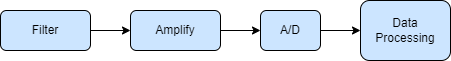
\includegraphics[width=0.55\linewidth]{graphics/acquisition_flow}
	\caption{Flow diagram voor het data acquisition van de bioreactor DO sensor}
	\label{fig:acq_flow}
\end{figure}


\subsubsection{Programma van Eisen}
Samen met de opdrachtgever, vertegenwoordigd door het engineeringsteam van Getinge, zijn er eisen aan het systeem gesteld. Voor het pakket van eisen zal een apart document worden gemaakt waar de aanpassingen door de tijd heen ook worden vastgelegd. In tabel \ref{tab:PakketvanEisen} zijn de eerste eisen van het project weergegeven. 

\begin{table}[H]
	\centering
	\caption{Programma van eisen.}
	\label{tab:PakketvanEisen}
	\begin{tabular}{clc}
		\toprule
		nr. & omschrijving  & opmerking \\ 
		\midrule
		1 & \makecell[l]{De sensorcomputer kan de DO sensor uitlezen met een sample \\rate van minimaal 1 Hz} &   \\
		2 & \makecell[l]{De sensor receiver op de biocontroller kan minimaal 2 sensoren \\ontvangen op {\'e\'e}n receiver} &   \\
		3 & \makecell[l]{De sensorcomputer kan draadloos communiceren met een \\biocontroller op een afstand van minimaal 10 m} &  \\
		4 & \makecell[l]{De sensorcomputer kan minimaal 28 dagen functioneren op \\accuvermogen} & \makecell[l]{Accu afmetingen mogen\\ niet te groot zijn (eis 6)} \\
		5 & \makecell[l]{De sensorcomputer kan worden gevoed via een accu en een \\tweede voedingsbron} & \makecell[l]{2de voeding voor\\ langdurig testen}\\
		6 & \makecell[l]{Het sensorsysteem past op de 3L bioreactor} &  \\
		7 & \makecell[l]{Het systeem is voorzien van een status indicatie van de batterij} & \\
		8 & \makecell[l]{Het systeem is van buitenaf uit/aan te schakelen} & \\
		9 & \makecell[l]{De sensorcomputer verstuurt de data via het huidige protocol} & \\
		10 & \makecell[l]{Het systeem maakt gebruik van de bestaande behuizing} & \\ 
		11 & \makecell[l]{De DO kan met een nauwkeurigheid van +- 1nA over de range \\van 0-340nA worden gemeten} & \\
		12 & \makecell[l]{De DO heeft een precisie van +- 0.5nA} & \\
		13 & \makecell[l]{De sensorcomputer verstuurd de sensor data met minimaal vier \\decimalen door naar de biocontroller} & \\		
		\bottomrule
	\end{tabular}
\end{table}

Er zal een testplan worden opgesteld om te kunnen bepalen of er aan de eisen is voldaan. 